\documentclass[aspectratio=169,10pt]{beamer}
% Shared preamble for the main deck and the backup deck.
% Compile with lualatex (see README.md).
\usetheme[progressbar=frametitle,numbering=fraction,sectionpage=progressbar]{metropolis}
\usepackage{fontspec}
\usepackage{unicode-math}
\setsansfont{Fira Sans}[BoldFont={Fira Sans SemiBold}, ItalicFont={Fira Sans Italic}, BoldItalicFont={Fira Sans SemiBold Italic}]
\setmonofont{Fira Mono}[Scale=0.9]
\setmathfont{Fira Math}
\usepackage{tikz}
\usetikzlibrary{arrows.meta,positioning,calc,shapes.geometric,fit,backgrounds,decorations.pathreplacing}
\usepackage{pgfplots}
\pgfplotsset{compat=1.18}
\usepackage{booktabs}
\usepackage{tabularx}
\usepackage{array}
\usepackage{xcolor}
\usepackage{fontawesome5}

% ---- palette -------------------------------------------------------------
\definecolor{ink}{HTML}{1F2A3A}      % text
\definecolor{navy}{HTML}{23395B}     % frame titles
\definecolor{blue}{HTML}{2F6DB5}     % main data colour (history, popular, known)
\definecolor{teal}{HTML}{1F8A70}     % method / good
\definecolor{orange}{HTML}{D9622B}   % cold start / warning / target
\definecolor{sand}{HTML}{F3EEE6}     % boxes
\definecolor{mist}{HTML}{E8EEF5}     % light blue boxes
\definecolor{grey}{HTML}{7A8494}

\setbeamercolor{normal text}{fg=ink,bg=white}
\setbeamercolor{frametitle}{bg=navy,fg=white}
\setbeamercolor{progress bar}{fg=orange,bg=navy!40}
\setbeamercolor{alerted text}{fg=orange}
\setbeamercolor{example text}{fg=teal}
\setbeamercolor{title separator}{fg=orange}
\metroset{block=fill}
\setbeamercolor{block title}{bg=mist,fg=navy}
\setbeamercolor{block body}{bg=mist!45,fg=ink}
\setbeamerfont{bibliography item}{size=\scriptsize}
\setbeamerfont{bibliography entry author}{size=\scriptsize}
\setbeamerfont{bibliography entry title}{size=\scriptsize}
\setbeamerfont{bibliography entry location}{size=\scriptsize}
\setbeamerfont{bibliography entry note}{size=\scriptsize}
\setbeamercolor{bibliography item}{fg=navy}
\setbeamercolor{bibliography entry author}{fg=ink}
\setbeamercolor{bibliography entry title}{fg=ink}
\setbeamercolor{bibliography entry location}{fg=ink}
\setbeamercolor{footnote}{fg=grey}
\setbeamerfont{footnote}{size=\tiny}
\setbeamerfont{frametitle}{size=\large}
\setbeamertemplate{itemize item}{\color{orange}\textbullet}
\setbeamertemplate{itemize subitem}{\color{grey}--}
\setlength{\leftmargini}{1.1em}

% ---- helpers ---------------------------------------------------------------
\newcommand{\code}[1]{\texttt{#1}}
% source line at the bottom of a frame
\newcommand{\source}[1]{\par\vfill\hfill{\scriptsize\color{grey}#1}}
% big number tile: \stat{value}{label}
\newcommand{\stat}[2]{%
  \begin{tikzpicture}
    \node[fill=mist,rounded corners=3pt,minimum width=2.55cm,minimum height=1.75cm,align=center,inner sep=4pt]
      {{\Large\bfseries\color{navy}#1}\\[2pt]{\scriptsize\color{ink}#2}};
  \end{tikzpicture}}
% one-line takeaway box at the bottom of a slide
\newcommand{\takeaway}[1]{%
  \par\vspace{4pt}\noindent
  \begin{tikzpicture}
    \node[fill=sand,draw=orange,line width=0.6pt,rounded corners=3pt,text width=0.92\textwidth,inner sep=6pt,align=left]
      {\small\textbf{\color{orange}Takeaway.} #1};
  \end{tikzpicture}}
\newcommand{\done}{{\color{teal}\faCheckCircle\ done}}
\newcommand{\planned}{{\color{orange}\faClock[regular]\ planned}}

\tikzset{
  box/.style={draw=navy,rounded corners=3pt,fill=mist,align=center,inner sep=4pt,font=\small},
  arr/.style={-{Stealth[length=2.2mm]},thick,color=navy},
  tok/.style={circle,draw=navy,thick,minimum size=7mm,inner sep=0pt,font=\scriptsize\bfseries},
  user/.style={rectangle,align=center,rounded corners=2pt,draw=grey,fill=white,minimum size=6mm,inner sep=1pt,font=\scriptsize},
}

\title{Next-Token Recommendation for Decentralized-Exchange Traders}
\author{Gergely Madarász \and Levente Tóth \and Béla Jakab}
\institute{Budapest University of Technology and Economics\\Advanced Machine Learning, project plan}
\date{October 2026}

\subtitle{Backup slides: literature takeaways, supplementary material, anticipated questions}

% question / answer helpers
\newcommand{\Q}[1]{\par{\color{orange}\bfseries Q.\ #1}\par\smallskip}
\newcommand{\A}{{\color{teal}\bfseries A.}\ }
\newcommand{\toindex}{\hfill\hyperlink{index}{\beamerreturnbutton{index}}}
\newcommand{\qsep}{\par\medskip{\color{grey!40}\hrule}\medskip}

\begin{document}

% ===========================================================================
\maketitle

\begin{frame}[label=index]{Index}
  \footnotesize
  \begin{columns}[T]
    \begin{column}{0.31\textwidth}
      \textbf{A. Literature review: main takeaways}
      \begin{itemize}\setlength{\itemsep}{0pt}
        \item \hyperlink{litsum}{Seven takeaways}
        \item \hyperlink{sarwar}{Sarwar 2001},
              \hyperlink{cremonesi}{Cremonesi 2010},
              \hyperlink{schein}{Schein 2002} in detail
        \item \hyperlink{others}{The other 18 references}
        \item \hyperlink{insights}{Insight $\rightarrow$ consequence table}
        \item \hyperlink{nlp}{The plan read with NLP vocabulary}
      \end{itemize}
    \end{column}
    \begin{column}{0.31\textwidth}
      \textbf{B. Supplementary material}
      \begin{itemize}\setlength{\itemsep}{0pt}
        \item \hyperlink{data}{Data, periods, descriptive statistics}
        \item \hyperlink{points}{Evaluation-point sizes}
        \item \hyperlink{baseline}{Full baseline results}
        \item \hyperlink{metrics}{Metric definitions},
              \hyperlink{stats}{statistics}
        \item \hyperlink{leak}{All leakage risks and controls}
        \item \hyperlink{ranker}{Method steps, ranker features}
        \item \hyperlink{expect}{Expectations and risks}
        \item \hyperlink{explor}{Exploratory follow-up (not in the plan)}
        \item \hyperlink{repro}{Reproducibility and provenance}
      \end{itemize}
    \end{column}
    \begin{column}{0.34\textwidth}
      \textbf{C. Anticipated hard questions}
      \begin{enumerate}\setlength{\itemsep}{0pt}
        \item \hyperlink{qframe}{Framing and usefulness}
        \item \hyperlink{qdata}{Data and labels}
        \item \hyperlink{qbots}{Accounts, bots, people}
        \item \hyperlink{qsplit}{Split and leakage}
        \item \hyperlink{qeval}{Metric and evaluation}
        \item \hyperlink{qstats}{Statistics}
        \item \hyperlink{qmath}{The similarity, as linear algebra}
        \item \hyperlink{qmodel}{Choice of models}
        \item \hyperlink{qnlp}{Questions from an NLP point of view}
        \item \hyperlink{qlit}{Literature and novelty}
        \item \hyperlink{qproj}{The project itself}
      \end{enumerate}
      \vspace{4pt}
      {\scriptsize\color{grey} Every slide has an \emph{index} button. Numbers are from the project plan unless marked otherwise.}
    \end{column}
  \end{columns}
\end{frame}

% ===========================================================================
\section{A. Literature review: main takeaways}

\begin{frame}[label=litsum]{Seven takeaways from the literature \toindex}
  \footnotesize
  \begin{enumerate}
    \setlength{\itemsep}{1pt}
    \item \textbf{Trades are implicit feedback.} Only positives are observed; absence is not dislike. Use ranking metrics and models built for implicit data \cite{hu2008,rendle2009}.
    \item \textbf{With short histories, item-to-item methods are the practical choice} \cite{sarwar2001,hidasi2016,ludewig2018}.
    \item \textbf{Simple, tuned methods are hard to beat.} Neural recommenders often fail to beat neighbour, linear or factorization models when those are tuned \cite{dacrema2019,rendle2020,rendle2021,anelli2022}.
    \item \textbf{Popularity is a strong baseline, and it is easy to measure it badly.} Measure it at the time of the recommendation \cite{ji2020pop}; in next-basket settings gains over frequency baselines are ``modest or even absent'' \cite{li2021}.
    \item \textbf{Repeat items and new items are different tasks} \cite{li2021}.
    \item \textbf{Evaluation choices change conclusions.} Per-user splits leak the future \cite{ji2020leak}; the split can reorder models \cite{meng2020}; sampled metrics can reverse comparisons \cite{krichene2020}; popular items dominate top-$N$ accuracy \cite{cremonesi2010}.
    \item \textbf{New items need content; two stages scale.} Cold start needs item attributes and trivial-heuristic references \cite{schein2002}; candidates, then a learned ranker \cite{covington2016,burges2010}.
  \end{enumerate}
  {\scriptsize\color{grey} Gap: no paper found that recommends fungible tokens from on-chain trades (four searches; NFT work exists \cite{choi2024,nftmine2023}).}
\end{frame}

\begin{frame}[label=sarwar]{Read in full: Sarwar, Karypis, Konstan, Riedl \cite{sarwar2001} \toindex}
  \footnotesize
  \begin{columns}[T]
    \begin{column}{0.49\textwidth}
      \textbf{Problem.} User-based neighbours search similar users at request time: slow, and sparse users rarely overlap.
      \par\medskip
      \textbf{Method.} Item--item similarities from the columns of the user--item matrix; keep the $k$ most similar items (``model size''); predict as a similarity-weighted sum over the user's items. Similarities compared: cosine, Pearson, adjusted cosine.
      \par\medskip
      \textbf{Experiments.} MovieLens, 100k ratings, 943 users with $\geq$20 ratings, 1{,}682 films; random 80/20 split; MAE.
    \end{column}
    \begin{column}{0.49\textwidth}
      \textbf{Findings.} Adjusted cosine is best. Item-based beats user-based everywhere, but ``not significantly large'' (MAE 0.726 vs 0.732). Flat after $\sim$30 neighbours. Keeping 25--50 neighbours (1.9--3\% of items) keeps 96--98.3\% of the accuracy.
      \par\medskip
      {\color{teal}\textbf{We take:}} the method; short neighbour lists.
      \par\medskip
      {\color{orange}\textbf{Does not carry over:}}
      (i) ratings and MAE vs.\ our binary ranking (adjusted cosine needs ratings, so we use cosine);
      (ii) $\geq$20 ratings per user vs.\ our median of 1;
      (iii) random split, not time;
      (iv) ``the item neighborhood is fairly static'': doubtful in a token market.
    \end{column}
  \end{columns}
\end{frame}

\begin{frame}[label=cremonesi]{Read in full: Cremonesi, Koren, Turrin \cite{cremonesi2010} \toindex}
  \footnotesize
  \begin{columns}[T]
    \begin{column}{0.49\textwidth}
      \textbf{Problem.} Recommenders were compared by rating error (RMSE), while users see a short list.
      \par\medskip
      \textbf{Evaluation.} Netflix (480{,}189 users, 17{,}770 items), MovieLens (6{,}040 / 3{,}883). Each held-out 5-star rating is ranked among 1{,}000 random unrated items; recall@$N$, precision@$N$. Test set split into the ``short head'' (popular items with a third of ratings; 1.7\% of Netflix items) and the ``long tail''.
    \end{column}
    \begin{column}{0.49\textwidth}
      \textbf{Findings.} (i) No simple relation between RMSE and top-$N$ accuracy. (ii) Most-popular is close to strong models on the full test set (MovieLens recall@10 $\approx$ 0.29 vs 0.28). (iii) On the long tail popularity collapses. (iv) PureSVD best throughout; an unnormalized cosine item-neighbour model with shrinkage is second on MovieLens.
      \par\medskip
      {\color{teal}\textbf{We take:}} popularity as a serious reference; the unnormalized sum of shrunk cosines; results also without the most popular tokens.
      \par\medskip
      {\color{orange}\textbf{Does not carry over:}} sampled negatives (we rank all, \cite{krichene2020}); random split; explicit ratings; the neighbour model is weaker on the Netflix long tail.
    \end{column}
  \end{columns}
\end{frame}

\begin{frame}[label=schein]{Read in full: Schein, Popescul, Ungar, Pennock \cite{schein2002} \toindex}
  \footnotesize
  \begin{columns}[T]
    \begin{column}{0.49\textwidth}
      \textbf{Problem.} Recommending items nobody has rated. Pure collaborative filtering ``cannot help in a cold-start setting''.
      \par\medskip
      \textbf{Method.} A latent-class (aspect) model where a class generates the \emph{actors} of a film; a new film is ``folded in'' through its cast. Compared with naive Bayes on the same content.
      \par\medskip
      \textbf{Experiments.} MovieLens + IMDb casts; films (not ratings) split at random: 331 of 1{,}682 unseen in training. Metrics: global ROC (GROC) and customer ROC (CROC, same number of recommendations per user).
    \end{column}
    \begin{column}{0.49\textwidth}
      \textbf{Findings.} On implicit prediction the aspect model beats naive Bayes; a trivial ``rank users by activity'' heuristic ties it on GROC (0.747 vs 0.743). The two curves can disagree; heuristics should always be reported.
      \par\medskip
      {\color{teal}\textbf{We take:}} cold start needs item attributes (for a token: launch pool, base currency, deployer, first trades); our metric gives every user 10 items (the CROC setting); compare with trivial heuristics.
      \par\medskip
      {\color{orange}\textbf{Does not carry over:}} their cold items are a random subset of an old catalogue with rich content; ours are new in time, continuous, with almost no content. How \emph{early} a new item can be recommended is not addressed.
    \end{column}
  \end{columns}
\end{frame}

\begin{frame}[label=others]{The other references, one line each \toindex}
  \scriptsize
  \renewcommand{\arraystretch}{1.3}
  \begin{tabularx}{\textwidth}{@{}>{\raggedright\arraybackslash}p{2.6cm}>{\raggedright\arraybackslash}X>{\raggedright\arraybackslash}p{2.0cm}@{}}
    \toprule
    Reference & Main point used & Read \\
    \midrule
    \cite{hu2008} & Implicit data as preferences with confidence; weighted MF by alternating least squares (iALS) & abstract \\
    \cite{rendle2009} & BPR: optimize a pairwise ranking criterion directly & abstract \\
    \cite{steck2019} & EASE: linear item--item model with closed form; competitive on sparse data & abstract \\
    \cite{hidasi2016} & Short sessions make MF inaccurate; practice falls back on item-to-item; GRU4Rec & abstract \\
    \cite{dacrema2019} & 7 of 18 neural recommenders reproducible; 6 of those beaten by simple heuristics & abstract \\
    \cite{rendle2020,rendle2021} & Tuned dot product beats NCF; tuned iALS competitive with later methods & abstract \\
    \cite{anelli2022} & 10 algorithms, 3 datasets: no consistent winner; no neural model best on accuracy & abstract \\
    \bottomrule
  \end{tabularx}
\end{frame}

\begin{frame}{The other references, one line each (cont.) \toindex}
  \scriptsize
  \renewcommand{\arraystretch}{1.3}
  \begin{tabularx}{\textwidth}{@{}>{\raggedright\arraybackslash}p{2.6cm}>{\raggedright\arraybackslash}X>{\raggedright\arraybackslash}p{2.0cm}@{}}
    \toprule
    Reference & Main point used & Read \\
    \midrule
    \cite{ludewig2018} & Session-based: nearest neighbours ``often perform equally well or significantly better'' than RNNs & abstract \\
    \cite{li2021} & Next basket: repeat vs explore are different; gains over frequency ``modest or even absent'' & abstract + concl. \\
    \cite{ji2020pop} & Popularity measured at recommendation time improves it by $\geq$70\% on MovieLens & abstract \\
    \cite{ji2020leak} & Leave-one-out per user leaks the future; use one global timeline & abstract \\
    \cite{meng2020} & The splitting strategy can change the ranking of models & abstract \\
    \cite{krichene2020} & Sampled metrics are inconsistent with exact ones; rank against all items & abstract \\
    \cite{burges2010} & RankNet $\rightarrow$ LambdaRank $\rightarrow$ LambdaMART: gradients scaled by $\Delta$NDCG & main sections \\
    \cite{covington2016} & Two stages (candidates, ranking); example age as a feature; avoid leaking the future & overview + concl. \\
    \cite{choi2024,nftmine2023} & NFT recommenders; item features help; NFT.mine reports AUC, not a time-split ranking metric & abstract + concl. \\
    \bottomrule
  \end{tabularx}
\end{frame}

\begin{frame}[label=insights]{Insight $\rightarrow$ consequence for the plan (full table) \toindex}
  \scriptsize
  \renewcommand{\arraystretch}{1.0}
  \begin{tabularx}{\textwidth}{@{}>{\raggedright\arraybackslash}X>{\raggedright\arraybackslash}X>{\raggedright\arraybackslash}p{2.9cm}@{}}
    \toprule
    Insight & Consequence for this project & Source \\
    \midrule
    Only positives are observed & Binary interactions, ranking metrics, implicit-feedback models & \cite{hu2008,rendle2009} \\
    Short histories favour item-to-item methods & Item neighbours first; most users have one item & \cite{sarwar2001,hidasi2016,ludewig2018} \\
    Simple tuned models match complex ones & No neural model; tuned iALS and EASE optional & \cite{dacrema2019,rendle2020,rendle2021,anelli2022} \\
    Popularity is strong and often mishandled & Fixed baseline, computed at $t$ from the history only & \cite{li2021,ji2020pop} \\
    Popularity depends on when it is measured & Time weighting is a core problem & \cite{ji2020pop}; own data \\
    Popular items dominate top-$N$ accuracy & Results also without the most popular tokens & \cite{cremonesi2010} \\
    A short neighbour list per item is enough & Top-$k$ truncation of similarities & \cite{sarwar2001} \\
    Generate candidates cheaply, rank with a learned model & Two-stage method with learned ranker & \cite{covington2016,burges2010} \\
    Repeat and explore are different tasks & New tokens primary; repeats separate & \cite{li2021} \\
    Per-user splits leak the future & One global timeline & \cite{ji2020leak} \\
    The split changes conclusions & Many evaluation points, spread reported & \cite{meng2020}; own data \\
    Sampled metrics mislead & Every model ranks all tokens & \cite{krichene2020} \\
    Cold start needs content and trivial references & Token features, refreshed lists, heuristics & \cite{schein2002,choi2024} \\
    \bottomrule
  \end{tabularx}
\end{frame}

\begin{frame}[label=nlp]{The plan in NLP vocabulary (an analogy, not a claim) \toindex}
  \footnotesize
  \renewcommand{\arraystretch}{1.12}
  \begin{tabularx}{\textwidth}{@{}>{\raggedright\arraybackslash}p{3.6cm}>{\raggedright\arraybackslash}p{3.8cm}>{\raggedright\arraybackslash}X@{}}
    \toprule
    In our plan & In NLP & Where the analogy breaks \\
    \midrule
    Popularity baseline & Unigram model & We predict \emph{unseen} items per user, not the next word \\
    Item--item cosine of co-usage & Distributional similarity from co-occurrence \cite{churchhanks1990} & ``Context'' is an account, not a window of words \\
    Heavy-tailed users per token & Zipf-like word frequencies & Our ``vocabulary'' grows every hour \\
    Cold-start tokens & Out-of-vocabulary words & No spelling to back off to; only launch metadata \\
    One account's history & A sentence & Median length 1; order mostly irrelevant for a 2-day set \\
    Learned ranker over signals & Re-ranking $n$-best lists with features & Few ``documents'' (10 dev points) \\
    \bottomrule
  \end{tabularx}
  \source{Extra references (not in the plan): Church \& Hanks 1990; Levy \& Goldberg 2014; Levy et al.\ 2015. See the last slides.}
\end{frame}

% ===========================================================================
\section{B. Supplementary material}

\begin{frame}[label=data]{Data: source, periods and sizes \toindex}
  \scriptsize
  \renewcommand{\arraystretch}{1.15}
  \begin{tabularx}{\textwidth}{@{}>{\bfseries}p{2.2cm}>{\raggedright\arraybackslash}X@{}}
    \toprule
    Source & Ethereum mainnet via free public RPC endpoints (\code{eth.drpc.org} for logs, \code{ethereum-rpc.publicnode.com} for transactions). No key, no licence restriction. \\
    Content & Every \code{Swap} event of Uniswap V2 and V3 style pools (incl.\ forks such as SushiSwap), the signing account, the two tokens of each pool. \\
    Row & \code{block, tx\_index, log\_index, timestamp, tx\_hash, tx\_from} (user), \code{tx\_to, pool, version, sender, recipient, amount0, amount1}. \\
    Feasibility & Blocks 26{,}049{,}600--26{,}150{,}399 (24 Sep--8 Oct 2026): 2{,}710{,}140 swaps, 1{,}965{,}611 tx, 211{,}547 accounts, 24{,}630 pools, 20{,}014 tokens, $\sim$440 MB Parquet, $\sim$2 h download. \\
    Not included & Uniswap V4, Curve, Balancer; prices; anything about a user beyond its trades. \\
    \bottomrule
  \end{tabularx}
  \vspace{2pt}
  \begin{tabularx}{\textwidth}{@{}p{3.4cm}p{3.4cm}p{2.2cm}>{\raggedright\arraybackslash}X@{}}
    \toprule
    Part & Blocks & Dates (2026) & Status and use \\
    \midrule
    \textbf{Project data, 12 weeks} & 25{,}344{,}000--25{,}948{,}799 & 18 Jun--10 Sep & To download; all tuning, selection, test. $\approx$16 M swaps, 2.5--3 GB \\
    Two weeks before feasibility & 25{,}948{,}800--26{,}049{,}599 & 10--24 Sep & Downloaded; used to check the baseline on a longer window \\
    Feasibility window & 26{,}049{,}600--26{,}150{,}399 & 24 Sep--8 Oct & Exploration only \\
    \bottomrule
  \end{tabularx}
  \source{604{,}800 blocks $\times$ 12 s = 84 days. Download cost: 20 min to 1.5 h per week, no fee.}
\end{frame}

\begin{frame}{Descriptive statistics \toindex}
  \footnotesize
  \begin{columns}[T]
    \begin{column}{0.5\textwidth}
      \textbf{Raw data, pools as items}\par\smallskip
      \begin{tabular}{@{}lr@{}}
        \toprule
        Distinct user--pool pairs & 719{,}752 (0.014\%) \\
        Median pools per user & 1 \\
        Users with one pool & 56\% \\
        Users with $\geq$5 pools & 21{,}990 \\
        Pools with $<$5 users & 70\% \\
        Swaps in top 10 / 100 pools & 29\% / 59\% \\
        Swaps by top 100 / 1{,}000 users & 27\% / 57\% \\
        Tx touching $>$1 pool & 20\% (41\% of swaps) \\
        \bottomrule
      \end{tabular}
    \end{column}
    \begin{column}{0.44\textwidth}
      \textbf{After preprocessing, tokens as items}\par\smallskip
      \begin{tabular}{@{}lr@{}}
        \toprule
        Users with $\geq$1 token & 157{,}060 \\
        Tokens & 19{,}631 \\
        Users with $\geq$2 / $\geq$5 tokens & 47{,}280 / 11{,}000 \\
        Tokens with $\geq$5 / $\geq$100 users & 4{,}655 / 606 \\
        Share of buys among legs & 52\% \\
        \bottomrule
      \end{tabular}
    \end{column}
  \end{columns}
  \par\medskip
  \textbf{Validation:} 99.1\% of blocks have a swap; no duplicate (\code{tx\_hash}, \code{log\_index}); no missing values; tokens read for 24{,}620 of 24{,}630 pools (99.98\% of swaps); 164k--225k swaps and 21.7k--30.5k users per full day.
\end{frame}

\begin{frame}{Skew of the raw data \toindex}
  \centering
  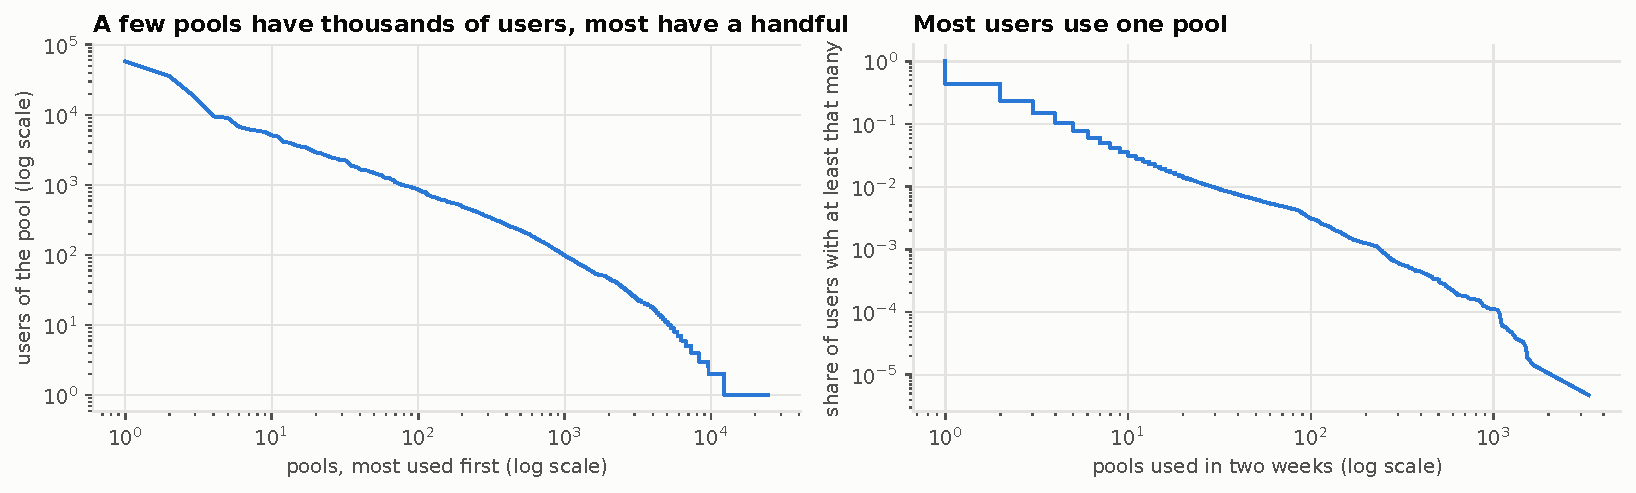
\includegraphics[width=\textwidth]{fig/token_rec_skew.pdf}
  \par\small\color{grey} Left: users per pool, most used pool first. Right: share of users with at least $n$ pools. Both axes logarithmic. Figure from the project plan (notebook 05).
\end{frame}

\begin{frame}[label=points]{Sizes at each evaluation point of the feasibility study \toindex}
  \small
  \centering
  \begin{tabular}{@{}llrrrrr@{}}
    \toprule
    Point & Use & Users in & Tokens in & Users & New pairs & Token absent \\
          &     & history  & history   & evaluated & to predict & from history \\
    \midrule
    after day 4 & dev & 60{,}994 & 9{,}933 & 8{,}037 & 27{,}349 & 14.9\% \\
    after day 5 & dev & 72{,}173 & 10{,}699 & 7{,}351 & 26{,}438 & 21.9\% \\
    after day 6 & dev & 84{,}534 & 11{,}723 & 7{,}073 & 26{,}223 & 21.6\% \\
    after day 7 & dev & 93{,}907 & 12{,}572 & 6{,}684 & 25{,}972 & 20.3\% \\
    after day 8 & dev & 103{,}268 & 13{,}240 & 7{,}237 & 23{,}573 & 20.1\% \\
    after day 9 & dev & 110{,}649 & 14{,}701 & 8{,}131 & 25{,}650 & 24.8\% \\
    after day 10 & dev & 119{,}785 & 17{,}530 & 8{,}403 & 24{,}583 & 24.0\% \\
    after day 12 & test & 138{,}501 & 18{,}701 & 8{,}604 & 23{,}138 & 21.7\% \\
    \bottomrule
  \end{tabular}
  \par\medskip
  \raggedright\small
  \begin{itemize}
    \item Feasibility split: train days 1--10, dev 11--12, test 13--14; seven rolling dev points.
    \item Weaknesses, both removed in the project: neighbouring targets overlap by one day; the test point was looked at during exploration.
  \end{itemize}
\end{frame}

\begin{frame}[label=baseline]{The baseline: full results \toindex}
  \scriptsize
  \begin{columns}[T]
    \begin{column}{0.55\textwidth}
      \begin{tabular}{@{}lrrrrrr@{}}
        \toprule
        Dev, 7 points & R@10 & low & high & NDCG & Hit & Cov. \\
        \midrule
        \textbf{Popularity} & \textbf{0.155} & 0.114 & 0.201 & 0.094 & 0.271 & 0.7\% \\
        Recent (last day) & 0.156 & 0.100 & 0.197 & 0.096 & 0.269 & 0.6\% \\
        \midrule
        Test (after day 12) & R@10 & & & NDCG & Hit & \\
        \midrule
        \textbf{Popularity} & \textbf{0.202} & & & 0.111 & 0.289 & \\
        Recent (last day) & 0.173 & & & 0.098 & 0.254 & \\
        \bottomrule
      \end{tabular}
      \par\medskip
      \begin{tabular}{@{}lrrrrrrrr@{}}
        \toprule
        after day & 4 & 5 & 6 & 7 & 8 & 9 & 10 & 12 \\
        \midrule
        Popularity & .201 & .185 & .161 & .157 & .128 & .114 & .142 & .202 \\
        Recent & .197 & .186 & .150 & .155 & .122 & .100 & .181 & .173 \\
        \bottomrule
      \end{tabular}
    \end{column}
    \begin{column}{0.42\textwidth}
      \begin{itemize}
        \item \textbf{By history size} (dev pooled): 0.179 with 1 token (16{,}077 evaluations), 0.183 with 2--4 (15{,}438), 0.117 with 5+ (21{,}401).
        \item \textbf{Variants:} first-time buys only 0.153; without the 5\% largest histories 0.161.
        \item \textbf{With repeats included:} the user's own history 0.270 beats popularity 0.166 \cite{li2021}. Not pursued.
        \item \textbf{One point misleads:} after day 10 recency wins by 0.04 with tight intervals; over 7 points it wins twice; at test it loses by 0.03.
        \item \textbf{Sampling interval} over users at one point: $\approx\pm0.007$.
      \end{itemize}
    \end{column}
  \end{columns}
\end{frame}

\begin{frame}[label=metrics]{Metric definitions \toindex}
  \small
  For account $u$ at point $t$: $L_u$ = its list of 10, $T_u$ = tokens it trades for the first time in $(t, t+2\text{ days}]$, $\mathcal{U}_t$ = evaluated accounts ($\geq$1 token in history, $|T_u|\geq1$).
  \begin{align*}
    \text{Recall@10} &= \frac{1}{|\mathcal{U}_t|}\sum_{u}\frac{|L_u\cap T_u|}{|T_u|}
    &
    \text{HitRate@10} &= \frac{1}{|\mathcal{U}_t|}\sum_{u}\mathbb{1}\left[\,|L_u\cap T_u|\geq1\,\right]
    \\
    \text{NDCG@10}(u) &= \frac{\sum_{k=1}^{10}\mathbb{1}[L_u^{(k)}\in T_u]/\log_2(k+1)}{\sum_{k=1}^{\min(10,|T_u|)}1/\log_2(k+1)}
    &
    \text{Coverage} &= \frac{|\bigcup_u L_u|}{|\text{tokens in history}|}
  \end{align*}
  \begin{itemize}
    \item Tokens absent from the history \textbf{stay in $T_u$}: they lower recall for every model equally.
    \item Reported per point, and as mean, lowest and highest over points.
    \item Also: by history size (1, 2--4, 5+), and with the most popular tokens (a third of the history's interactions) removed from $T_u$ \cite{cremonesi2010}.
  \end{itemize}
\end{frame}

\begin{frame}[label=stats]{Statistics of the comparison \toindex}
  \small
  \begin{columns}[T]
    \begin{column}{0.5\textwidth}
      \textbf{Paired by point.} $d_p = \text{R@10}_{\text{model}}(p) - \text{R@10}_{\text{base}}(p)$ for the 14 test points.
      \begin{itemize}
        \item \textbf{Primary:} mean $\bar d$ with a bootstrap interval over points; success if it excludes 0.
        \item \textbf{Secondary:} sign test on wins. Two-sided $p$ for $n=14$:
          \begin{tabular}{@{}lccc@{}}
            wins & 11 & 12 & 13 \\
            $p$ & 0.057 & \textbf{0.013} & 0.002 \\
          \end{tabular}
        \item \textbf{Within a point:} bootstrap over users (\code{bootstrap\_mean}); $\approx\pm0.007$.
      \end{itemize}
    \end{column}
    \begin{column}{0.47\textwidth}
      \textbf{Power of the sign test} (chance of $\geq$12 wins of 14 if the model truly wins a point with probability $q$):
      \par\smallskip
      \centering
      \begin{tabular}{@{}lccc@{}}
        \toprule
        $q$ & 0.7 & 0.8 & 0.9 \\
        power & 0.16 & 0.45 & 0.84 \\
        \bottomrule
      \end{tabular}
      \par\medskip\raggedright
      This is why the sign test is secondary: it only detects a model that wins almost every day. The mean difference uses the size of the gains, not only their sign.
      \par\smallskip
      {\color{grey}\scriptsize Computed for this deck; not in the plan.}
    \end{column}
  \end{columns}
\end{frame}

\begin{frame}[label=leak]{Leakage risks and controls (1/2) \toindex}
  \scriptsize
  \renewcommand{\arraystretch}{1.2}
  \begin{tabularx}{\textwidth}{@{}>{\raggedright\arraybackslash}p{6.0cm}>{\raggedright\arraybackslash}X@{}}
    \toprule
    Risk & Control \\
    \midrule
    Random or per-user leave-one-out split shows other users' future \cite{ji2020leak} & One global point in time per evaluation, for all users \\
    Users or items of the future enter the model & Indexed from the history only (\code{build\_task}, tested); future-only tokens count as misses \\
    Item statistics computed on all data & Popularity, recent popularity, token age from the history only \\
    Base-currency list uses the future & Decided on the first ten days; the same three tokens result from any cut \\
    Recommending what the user already has & The user's history is removed from the ranking \\
    Sampled negatives distort the comparison \cite{krichene2020} & Every model ranks all tokens of the history \\
    Tuning on test & Settings on Dev A, models on Dev B; test scored once from a frozen commit \\
    \bottomrule
  \end{tabularx}
\end{frame}

\begin{frame}{Leakage risks and controls (2/2) \toindex}
  \scriptsize
  \renewcommand{\arraystretch}{1.2}
  \begin{tabularx}{\textwidth}{@{}>{\raggedright\arraybackslash}p{6.0cm}>{\raggedright\arraybackslash}X@{}}
    \toprule
    Risk & Control \\
    \midrule
    Ranker learns from labels after the points it is scored on & Trained on Dev A only, which ends before Dev B and test; features use the history before each example's point \\
    Random cross-validation mixes rows of one period & Hyperparameters chosen by holding out whole evaluation points \\
    Overlapping targets make points look independent & Non-overlapping two-day targets in the project \\
    Pool tokens were read today, not at swap time & A pool's two tokens are immutable. Not a leak \\
    Evaluated users are chosen by their future (they trade something new) & Defines who is scored, not what a model sees. Reads: given that a user picks up something new, was it in the list? \\
    One person, several accounts & Not handled. Makes users look less active; cannot leak labels \\
    Trades before the data starts & Such tokens look ``new''; a longer history reduces this; not removed \\
    \bottomrule
  \end{tabularx}
\end{frame}

\begin{frame}[label=ranker]{Method steps and ranker features \toindex}
  \scriptsize
  \begin{columns}[T]
    \begin{column}{0.48\textwidth}
      \renewcommand{\arraystretch}{1.15}
      \begin{tabular}{@{}cp{2.3cm}p{2.3cm}@{}}
        \toprule
        Step & Model & Tuned on Dev A \\
        \midrule
        0 & Popularity (baseline) & nothing \\
        1 & Item neighbours & $k$, $\lambda$ \\
        2 & + popularity & weight $w$ \\
        3 & Time weighting & half-life $h$, history length \\
        4 & Cold start & refresh interval, features \\
        5 & Learned ranker & regularization; trees: number, depth, learning rate \\
        \bottomrule
      \end{tabular}
      \par\medskip
      \textbf{Status:} only step 0 has reported results. Steps 1--2 are implemented and tested in \code{pool\_recsys.py}.
      \par\medskip
      \textbf{Ranker models:} (1) logistic regression; (2) boosted trees, logistic loss; (3) boosted trees, LambdaMART (group = one user at one point) \cite{burges2010}.
    \end{column}
    \begin{column}{0.5\textwidth}
      \renewcommand{\arraystretch}{1.15}
      \begin{tabularx}{\textwidth}{@{}p{1.5cm}X>{\centering\arraybackslash}p{0.9cm}@{}}
        \toprule
        Group & Features of (user, candidate) & Core problem \\
        \midrule
        Popularity & users in whole history, last day, several half-lives & 2 \\
        Neighbours & $r_{ui}$, largest single similarity, number of user tokens pointing to it; plain and time-weighted & 1, 2 \\
        User & history size, time since last trade, share of buys & 1 \\
        Token & age, users in first hour and first day, base currency of launch pool & 3 \\
        \bottomrule
      \end{tabularx}
      \par\medskip
      \textbf{Candidates:} union of top tokens by popularity and by neighbour score, a few hundred. \textbf{Candidate recall} is measured first: it caps the ranker.
      \par\smallskip
      \textbf{Ablation:} drop one feature group at a time.
    \end{column}
  \end{columns}
\end{frame}

\begin{frame}[label=expect]{What to expect from each part of the work \toindex}
  \small
  \renewcommand{\arraystretch}{1.3}
  \begin{tabularx}{\textwidth}{@{}>{\raggedright\arraybackslash}p{3.0cm}>{\raggedright\arraybackslash}X>{\raggedright\arraybackslash}p{4.2cm}@{}}
    \toprule
    Work & What it can and cannot deliver & Basis \\
    \midrule
    More weeks, more points & No gain in score; the precondition for judging any model & Day-to-day range 0.11--0.20 \\
    Neighbours + popularity & Personal lists, much higher coverage; recall gain to be established & Baseline coverage $<$1\% \\
    Time weighting & More stable across periods; needed before 12 weeks of history help & Recency wins on some days only \\
    Cold start & Largest unreachable part; a model has minutes to hours of information & 15--25\% of the target \\
    Learned ranker & Gain where the best mix differs between users; capped by candidate recall & 0.18 vs 0.12 by history size \\
    \bottomrule
  \end{tabularx}
\end{frame}

\begin{frame}{Risks and mitigations (full table) \toindex}
  \small
  \renewcommand{\arraystretch}{1.15}
  \begin{tabularx}{\textwidth}{@{}>{\raggedright\arraybackslash}p{4.6cm}c>{\raggedright\arraybackslash}X@{}}
    \toprule
    Risk & Likelihood & Mitigation \\
    \midrule
    Method does not beat baseline & medium & Null result on 14 clean points is reportable; method contains the baseline \\
    Period effects larger than model effects & high & Paired per point; many points; spread reported \\
    Public endpoints slow or unavailable & medium & Resumable, chunked download; all data already exists \\
    Bots dominate evaluated users & medium & User-averaged metrics, binary interactions, results by history size \\
    Ranker overfits few periods & high & LR first, few features, shallow trees, held-out points, selection on Dev B \\
    Cold-start work does not fit in time & medium & Independent of other models; reported separately \\
    \bottomrule
  \end{tabularx}
\end{frame}

\begin{frame}[label=explor]{Exploratory follow-up on 28 days (not part of the plan) \toindex}
  \scriptsize
  \textbf{What it is.} After the plan, the same study was repeated on 28 days (10 Sep--8 Oct; 5.73 M swaps; 21 dev points), with \emph{nothing re-tuned} and untuned models. Source: \code{research/token\_recommendation\_28\_days.md}, notebook 08. It is \textbf{not} test evidence.
  \par\medskip
  \begin{columns}[T]
    \begin{column}{0.56\textwidth}
      \renewcommand{\arraystretch}{1.1}
      \begin{tabular}{@{}lrrr@{}}
        \toprule
        Model (21 dev points) & R@10 & vs base & wins \\
        \midrule
        Popularity (baseline) & 0.147 & & \\
        Recent popularity & 0.166 & +0.019 & 16/21 \\
        Item neighbours alone & 0.130 & $-$0.017 & 6/21 \\
        Truncated SVD, rank 32 & 0.121 & $-$0.026 & 3/21 \\
        Blend 50\% pop.\ + neighbours & 0.181 & +0.034 & 19/21 \\
        Blend 85\% recent + neighbours & 0.186 & +0.039 & 20/21 \\
        \bottomrule
      \end{tabular}
    \end{column}
    \begin{column}{0.42\textwidth}
      \begin{itemize}
        \item Blend vs baseline on the 11 points with separate targets: 10 wins, +0.036 (interval +0.022 to +0.051).
        \item Gain smaller than in two weeks (+0.051 $\rightarrow$ +0.034): seven points over-stated it.
        \item Recency matters more than two weeks suggested.
        \item Longer, unweighted history \emph{lowers} every model: supports time weighting as core problem 2.
        \item Unreachable share: 10--31\%.
      \end{itemize}
    \end{column}
  \end{columns}
  \source{Use only if asked for evidence. Note: the plan calls the 10--24 Sep data ``not used for evaluation''; this follow-up did score untuned models on it.}
\end{frame}

\begin{frame}[label=repro]{Reproducibility and provenance \toindex}
  \small
  \begin{itemize}
    \item \textbf{Code:} \code{dex\_swaps.py} (download), \code{pool\_recsys.py} (preprocessing, models, metrics; 18 tests), notebook \code{05\_pool\_recommendation\_data\_and\_baseline.ipynb} (every number of the plan).
    \item \code{python dex\_swaps.py --start 26049600 --blocks 100800}: about two hours; the notebook then runs in about two minutes. Random seeds fixed.
    \item \textbf{Data} are regenerated from the chain; they are not committed (about 440 MB).
    \item \textbf{Provenance:} the three authors chose the topic, developed the code and reviewed the process. An AI system (Claude Opus 5.5) assisted with the code, ran experiments and drafted the text under the authors' direction. The authors are responsible for the content.
    \item \textbf{Name:} the idea started as ``next-\emph{pool}'' recommendation; file names still say ``pool''.
  \end{itemize}
\end{frame}

% ===========================================================================
\section{C. Anticipated hard questions}

\begin{frame}[label=qframe]{1. Framing and usefulness \toindex}
  \footnotesize
  \Q{Why would anyone want this? Recommending speculative tokens to people seems harmful.}
  \A We agree that it is not obviously desirable as a product, and the plan says so. We treat the recommender as a \emph{measuring instrument}: how predictable is it which token an account adopts next, and how should such a fast-moving setting be evaluated. Only public, pseudonymous data is used. No prices or returns are predicted.
  \qsep
  \Q{Is this not price prediction in disguise?}
  \A No. The target is \emph{which} token an account trades for the first time, buy or sell. Prices are not in the data and not in the target. A token can be adopted while its price falls.
  \qsep
  \Q{Why two days and a list of ten? These look arbitrary.}
  \A They are choices, fixed before any model is run, so they cannot be tuned to make a model look good. Ten is a list a person can read; two days fits a fast market. One day, one week and lists of 20 or 50 are listed as extensions.
\end{frame}

\begin{frame}{1. Framing and usefulness (cont.) \toindex}
  \footnotesize
  \Q{Why do you exclude repeats? Half of what users do next is a repeat.}
  \A Repeat and new items are different tasks \cite{li2021}. Repeats are easy: the user's own history scores 0.270 against 0.166 for popularity. The question of interest is discovery, so new tokens are the primary task; the all-tokens task is reported only.
  \qsep
  \Q{Is recall@10 = 0.155 good or bad?}
  \A Alone it means little; it is the reference for the comparison. Two context points: (i) 15--25\% of the target is unreachable for any model of past trades, so the ceiling is roughly 0.75--0.85; (ii) numbers from other papers (e.g.\ 0.29 on MovieLens \cite{cremonesi2010}) are not comparable, because they rank against 1{,}000 sampled items, not all items.
  \qsep
  \Q{What would make you conclude the idea does not work?}
  \A The success criterion is fixed in advance: on 14 test points the paired interval of the recall@10 difference must exclude zero. If it does not, we report a null result. Since the method contains the baseline ($w=1$), we can also report \emph{which} signals add nothing.
\end{frame}

\begin{frame}[label=qdata]{2. Data and labels \toindex}
  \footnotesize
  \Q{A trade is not a preference. Selling a token is the opposite of liking it.}
  \A Correct: it is engagement, not preference, which is what implicit feedback means \cite{hu2008}. Both buys and sells count as ``the account dealt with this token''. We report a variant where only first-time \emph{buys} are the target: 0.153 vs 0.155. The conclusion does not change.
  \qsep
  \Q{How can an account sell a token it has never traded?}
  \A It acquired it before the data starts, or by a transfer, or on an exchange we do not cover. Then it looks ``new''. This is a known limitation; a longer history reduces it, it is not removed.
  \qsep
  \Q{Why remove WETH, USDC, USDT? People do pick them up.}
  \A They are money, not a choice: WETH is in the trades of 81\% of accounts. Recommending them is trivial and would dominate every list. The rule ($>$10\% of accounts) was set on the training days; there is a wide gap between the 3rd token (29\%) and the 4th (5\%), so any threshold in between gives the same three. Its sensitivity was not tested.
\end{frame}

\begin{frame}{2. Data and labels (cont.) \toindex}
  \footnotesize
  \Q{Only Uniswap V2/V3 on Ethereum. Is that representative?}
  \A No, and we do not claim it is. A token bought on Uniswap V4, Curve or an aggregator looks new to us. The choice is pragmatic: the data are complete, free and structured. Other venues and chains (Base, Solana) are listed as extensions; there we would expect a larger cold-start share.
  \qsep
  \Q{Why measure popularity by distinct accounts, not by volume?}
  \A Volume is dominated by a few very active accounts and large traders. What we predict is \emph{accounts} adopting a token, so the matching statistic is how many accounts adopted it.
  \qsep
  \Q{Your median user has one token. Is that not just because the window is short?}
  \A Partly. A longer history gives more tokens per account, which is one reason for the 12 weeks. But a longer history also contains stale interest; this is why the length of the history and the time weighting are tuned, not assumed.
\end{frame}

\begin{frame}[label=qbots]{3. Accounts, bots, people \toindex}
  \footnotesize
  \Q{An address is not a person. And many accounts are bots.}
  \A Both true. (i) One person with several addresses is not handled; it makes histories look shorter and cannot leak labels. (ii) Bots: arbitrage cycles that end where they start leave no bought or sold token and drop out; interactions are binary; metrics average over accounts, so a bot with 10{,}000 swaps counts as much as a person with two; results are reported by history size. A separation of automated accounts is optional work.
  \qsep
  \Q{Sandwich bots buy and sell in two transactions; they are not cycles. They stay in.}
  \A Yes, such accounts stay in. They will mostly appear in the ``5+ tokens'' group, which is reported separately, so their effect is visible rather than hidden in an average.
  \qsep
  \Q{The signer is not always the trader: relayers and solvers sign for others.}
  \A Correct, and this is not addressed in the plan. For intent-based systems the signer is a solver acting for many users. Such accounts look like very active users; per-account averaging limits their weight. Honest answer: it is a source of noise in the user identity that we would have to measure.
\end{frame}

\begin{frame}[label=qsplit]{4. Split and leakage \toindex}
  \footnotesize
  \Q{Your test period lies before the data you explored. Is that a valid test?}
  \A It is untouched, but not later in time; the plan states this caveat. No \emph{data} leak is possible: every model is refit at each point from the history before it. What can leak is \emph{design insight} (the choice of the three core problems was made on later data). Testing on an earlier, unexamined period is the cleanest option available today without waiting for new blocks.
  \qsep
  \Q{You evaluate only accounts that trade something new. That selects on the future.}
  \A It selects \emph{who is scored}, not what the model sees. The metric reads: ``given that an account picks up something new, was it in its list?'' Recall is undefined for an account with no new token. All models are scored on the same accounts, so the comparison stays fair.
  \qsep
  \Q{Points share most of their history. They are not independent.}
  \A True. Non-overlapping targets remove the overlap of labels, but the histories and market regimes are correlated. We therefore report every point, not only a mean, and treat the bootstrap interval as approximate. A block bootstrap over consecutive points \cite{kunsch1989} would be the more cautious variant.
\end{frame}

\begin{frame}{4. Split and leakage (cont.) \toindex}
  \footnotesize
  \Q{Token age is computed from the first time you see the token. Old tokens look young at the start of the data.}
  \A Yes: it is left-censored. The 14-day burn-in means every point has at least 14 days of history; tokens first seen in the burn-in are ``at least that old''. It cannot leak future information, because it is computed from the history only.
  \qsep
  \Q{You will try many models on Dev B. That is multiple testing.}
  \A Model choice happens on Dev B, which is why it is separate from the test. On the test period the frozen chosen method is compared with the fixed baseline once, under a criterion written down in advance. Other models are reported descriptively.
  \qsep
  \Q{The ranker is trained on rows from 10 periods. A random cross-validation would look fine and be wrong.}
  \A Agreed, which is why hyperparameters and early stopping use cross-validation that holds out \emph{whole evaluation points}. Millions of rows are still only ten market situations.
\end{frame}

\begin{frame}[label=qeval]{5. Metric and evaluation \toindex}
  \footnotesize
  \Q{Unreachable tokens stay in the denominator. That punishes your models for something they cannot do.}
  \A Deliberately. Removing them would report a task easier than the real one. They lower every model by the same amount, so comparisons are unaffected; the reachable share is reported separately so the ceiling is visible.
  \qsep
  \Q{Why recall@10 and not NDCG, MAP or AUC?}
  \A Recall@10 has a plain reading (share of new tokens that were in the list), and with a list of fixed length it is the setting in which user-activity heuristics have no advantage \cite{schein2002}. NDCG@10 and hit rate are reported too. AUC over all items is dominated by the ordering of thousands of irrelevant tokens.
  \qsep
  \Q{The LambdaMART ranker optimizes NDCG, but your main metric is recall. Mismatch?}
  \A A small one. With binary relevance and 10 slots both reward putting true tokens in the list; NDCG also rewards putting them high. Both are reported. If the mismatch matters, it shows up in the selection on Dev B.
\end{frame}

\begin{frame}{5. Metric and evaluation (cont.) \toindex}
  \footnotesize
  \Q{Why rank against all tokens? Sampling 100 negatives is standard and cheaper.}
  \A Sampled metrics are inconsistent with exact ones and can reverse which model is better \cite{krichene2020}. With $\sim$20{,}000 tokens, scoring all is cheap with sparse matrices.
  \qsep
  \Q{Popularity is a straw man.}
  \A The literature says the opposite: popularity is close to strong models in top-$N$ evaluation \cite{cremonesi2010}, and gains over frequency baselines are often ``modest or even absent'' \cite{li2021}. We compute it carefully, at time $t$ \cite{ji2020pop}, and also report recent popularity, which is the stronger simple reference on some days.
  \qsep
  \Q{Coverage 0.7\%: why should we care?}
  \A It detects a degenerate recommender that shows everybody the same list. A model can raise recall by concentrating on a few popular tokens; coverage makes that visible.
\end{frame}

\begin{frame}[label=qstats]{6. Statistics \toindex}
  \footnotesize
  \Q{A sign test on 14 points has almost no power.}
  \A Correct: if the model truly wins a point with probability 0.8, the chance of $\geq$12 wins is only 0.45 (slide \hyperlink{stats}{statistics}). That is why the primary criterion is the \emph{mean} paired difference with a bootstrap interval; the sign test is a robust secondary check.
  \qsep
  \Q{A percentile bootstrap with 14 observations is unreliable.}
  \A It tends to be too narrow for small samples. We will report the per-point differences themselves, so a reader can apply any test. A paired $t$ interval and a block bootstrap \cite{kunsch1989} are natural cross-checks; with a clear effect they agree, and with a marginal one we would report the result as marginal.
  \qsep
  \Q{Points have different numbers of users. Should they get equal weight?}
  \A Yes, on purpose: the main source of variance is the market situation, not the sample of users (period range 0.11--0.20 vs $\pm0.007$ within a point). Each point is one observation of a market situation.
\end{frame}

\begin{frame}[label=qmath]{7. The similarity, as linear algebra \toindex}
  \small
  Let $X\in\{0,1\}^{m\times n}$ be the account--token matrix, $D=\mathrm{diag}(X^{\mathsf{T}} X)$ (users per token), $h_u$ the row of $u$.
  \Q{Write your model down. What is it, algebraically?}
  \A With $\lambda=0$ and no truncation: $S = D^{-1/2}X^{\mathsf{T}} X D^{-1/2}$ (cosine) and the scores are $r_u = h_u S$, a \emph{linear} map of the history vector. It is an item--item model like EASE \cite{steck2019}, whose matrix is learned instead: $B = I - P\,\mathrm{diagMat}(\mathbf{1}\oslash\mathrm{diag}(P))$, $P=(X^{\mathsf{T}} X+\lambda I)^{-1}$. PureSVD \cite{cremonesi2010} is the rank-$k$ case $r_u = h_u V_kV_k^{\mathsf{T}}$.
  \qsep
  \Q{With shrinkage and top-$k$ truncation, $S$ is no longer a cosine matrix, not PSD, not even symmetric. Is that a problem?}
  \A Without them $S$ is a Gram matrix, hence PSD. With them it is neither, and it does not need to be: $S$ is never used as a kernel or inverted, only to score and sort. All that matters is the order of $r_{ui}$ within each account.
\end{frame}

\begin{frame}{7. The similarity, as linear algebra (cont.) \toindex}
  \footnotesize
  \Q{You say the sum is ``not normalized''. Normalizing by $|H_u|$ would change nothing.}
  \A Right: dividing $r_u$ by any per-account constant leaves the account's ranking unchanged. The normalization we skip is the \emph{per-candidate} one of Sarwar et al.\ \cite{sarwar2001}, dividing by $\sum_j |s_{ji}|$; that changes the order. Without it, a token that many of the user's tokens point to ranks higher \cite{cremonesi2010}. Per-account scaling ($\tilde r$, max 1) matters only when blending with popularity.
  \qsep
  \Q{What is the shrinkage, statistically?}
  \A $|U_i\cap U_j|/(\sqrt{|U_i||U_j|}+\lambda)$ pulls the similarity of tokens with few users towards zero, like a prior that ``two thin tokens are probably unrelated''. With $|U_i|=|U_j|=|U_i\cap U_j|=1$ the plain cosine is 1, the maximum, on one shared account; $\lambda=10$ gives $1/11$.
  \qsep
  \Q{Why an exponential decay $2^{-a/h}$?}
  \A One parameter with a plain meaning (the half-life), and both references are its limits: $h\to\infty$ is all-time popularity, small $h$ approaches last-day popularity. A hard window is the other option and is covered by tuning the history length.
\end{frame}

\begin{frame}[label=qmodel]{8. Choice of models \toindex}
  \footnotesize
  \Q{This is an \emph{advanced} ML course. Why no deep learning?}
  \A Because the evidence says it is unlikely to help here: most accounts have one or two tokens, and on such data tuned simple models match or beat neural ones \cite{dacrema2019,anelli2022,ludewig2018}. The learning in the project is in the ranker (gradient-boosted trees with a LambdaMART objective \cite{burges2010}), and in an evaluation design that can tell a real gain from a lucky period.
  \qsep
  \Q{Why not matrix factorization? It handles sparsity.}
  \A User factors would be fitted on one or two interactions for most accounts. Variants without user factors (PureSVD, EASE) are item--item models, close to ours. Tuned iALS \cite{hu2008,rendle2021} and EASE \cite{steck2019} are optional references.
  \qsep
  \Q{Ten training periods for gradient-boosted trees? You will overfit.}
  \A That risk is rated high in the plan. Hence: logistic regression first (a handful of parameters), few features, shallow trees, validation on held-out points, selection on Dev B, and comparison with the best \emph{fixed} combination. If the trees do not beat it, the fixed combination is the answer.
\end{frame}

\begin{frame}{8. Choice of models (cont.) \toindex}
  \footnotesize
  \Q{Positives are a tiny minority of the ranker's rows. Class imbalance?}
  \A It matters for calibrated probabilities, not for rankings within an account. LambdaMART compares pairs within a group (one account at one point), so it is insensitive to the overall rate. For logistic regression, re-weighting the classes mainly shifts the intercept, which does not change the order within an account.
  \qsep
  \Q{What if the true token is not among the candidates?}
  \A Then no ranker can find it. Candidate recall is measured first and reported as the ceiling of stage 2.
  \qsep
  \Q{How can you recommend a token that does not exist yet?}
  \A Under the main protocol you cannot; it counts as a miss. Core problem 3 adds a second protocol in which lists are rebuilt every few hours inside the target window, with the baseline refreshed the same way. New tokens are then scored from features available within the first hour, and compared with trivial heuristics such as ``new tokens with the most early users'' \cite{schein2002}.
\end{frame}

\begin{frame}[label=qnlp]{9. Questions from an NLP point of view \toindex}
  \footnotesize
  \Q{Each account's history is a sentence of tokens. Why not train a language model or a transformer recommender?}
  \A The median ``sentence'' has length one, and the target is an unordered set over two days, not the next item. Sequential models such as SASRec \cite{kang2018} need sequences; in session-based recommendation, neighbour methods often equal or beat RNNs \cite{ludewig2018}.
  \qsep
  \Q{Why not learn embeddings (word2vec / item2vec)?}
  \A Skip-gram with negative sampling implicitly factorizes a shifted PMI matrix of co-occurrences \cite{levy2014}, and with tuned hyperparameters count-based methods match it \cite{levy2015}. Our cosine on co-usage is the count-based counterpart. Item2vec \cite{barkan2016} is a reasonable extension, but for an account with one token it reduces to an item--item similarity again.
  \qsep
  \Q{Why cosine and not PMI, the standard association measure \cite{churchhanks1990}?}
  \A $\mathrm{PMI}_{ij} = \log \bigl(N\,|U_i\cap U_j| \,/\, |U_i||U_j|\bigr)$ divides by the product of the counts, cosine by their geometric mean, so PMI favours rare pairs. Here rare means tokens with one or two accounts, where PMI is very noisy (the known low-count bias, cf.\ context smoothing in \cite{levy2015}). Shrinkage does the analogous job for cosine. Other similarities could be compared on Dev A.
\end{frame}

\begin{frame}{9. Questions from an NLP point of view (cont.) \toindex}
  \footnotesize
  \Q{Your user-per-token plot looks like Zipf's law. So what?}
  \A It is heavy-tailed in the same way: a few tokens are used by thousands of accounts, most by a handful. The consequences are the familiar ones: a frequency (unigram-like) baseline is strong, and the tail is where data are too thin. This is why we report results without the most popular tokens \cite{cremonesi2010}. We do not claim a specific power law; we have not fitted one.
  \qsep
  \Q{Cold start is the OOV problem. NLP solved it with subwords. What is your subword?}
  \A A token has no spelling to back off to. Its ``subword'' features are its metadata from the first minutes: launch pool and base currency, deploying account, number of early users, age. Whether that is enough is exactly core problem 3.
  \qsep
  \Q{Is ``next-token'' in your title a pun?}
  \A Only in English. ``Token'' here means a crypto asset, not a piece of text; the task is recommendation, not language modelling.
\end{frame}

\begin{frame}[label=qlit]{10. Literature and novelty \toindex}
  \footnotesize
  \Q{You read three papers in full. Is that a literature review?}
  \A The plan says this openly: three papers in full (the method, the evaluation, the cold start), the others at abstract level, some with conclusions. The others are cited only for claims stated in their abstracts. The reference list marks the reading depth of each.
  \qsep
  \Q{What is new? These are methods from 2001--2016.}
  \A The methods are not new, on purpose. What is new is the task: recommending fungible tokens from on-chain trading histories, for which our searches found no paper; the item definition (token, not pool); and an evaluation design for a market where the score changes by a factor of two from one day to the next. ``No paper found'' means four searches, not proof.
  \qsep
  \Q{The NFT recommenders \cite{choi2024,nftmine2023} solve the same problem.}
  \A NFTs are unique items with images and text; tokens are interchangeable with almost no content. And NFT.mine reports AUC against classifiers, not a ranking metric on a time split, so its numbers are not comparable with ours.
\end{frame}

\begin{frame}[label=qproj]{11. The project itself \toindex}
  \footnotesize
  \Q{What if the public endpoints stop working?}
  \A The download is resumable and chunked; a rate limit only slows it down. All the data already exists on the chain, and other public endpoints serve the same logs.
  \qsep
  \Q{Can you do all of this in one semester?}
  \A Work packages 1--3 are the core and produce a complete result (a tuned neighbour model compared with the baseline on clean points). Time weighting and cold start add to it; cold start depends only on the protocol and can be reported on its own. Factorization references and bot separation are optional.
  \qsep
  \Q{An AI system drafted the plan. Do you understand it?}
  \A The AI assisted with code, experiments and drafting under our direction, and the plan states this. We chose the topic, developed the code, reviewed the process, and are responsible for the content. The questions on these slides are the test of that.
\end{frame}

\begin{frame}{11. The project itself (cont.) \toindex}
  \footnotesize
  \Q{Do you have \emph{any} evidence the method can beat popularity?}
  \A Not in the plan, deliberately: seven overlapping points cannot separate a model effect from a period effect. An exploratory follow-up on 28 days with untuned models suggests a blend gains about +0.03 (slide \hyperlink{explor}{exploratory}). It is a hint, not a result.
  \qsep
  \Q{Why does the plan not report the neighbour model you already ran?}
  \A Untuned versions were run during exploration and stay in the notebook. Seven overlapping points, with a baseline that itself moves between 0.11 and 0.20, cannot tell a model effect from a period effect; reporting them would invite exactly the conclusion we cannot support.
  \qsep
  \Q{What gain do you expect, then?}
  \A No number is promised. The exploratory hint is about +0.03 recall@10. The success criterion asks only that the paired interval excludes zero, and a null result is an acceptable outcome.
\end{frame}

% ---------------------------------------------------------------------------
\begin{frame}[allowframebreaks,t]{References}
  \setbeamertemplate{bibliography item}{\insertbiblabel}
  \begin{thebibliography}{Covington 2016}
    \scriptsize
    % The 21 references of the project plan. Shared by both decks.
% \bibitem[label]{key}: the label is what \cite prints on the slides.
\bibitem[Hu 2008]{hu2008} Y.~Hu, Y.~Koren, C.~Volinsky. Collaborative filtering for implicit feedback datasets. \emph{ICDM}, 2008.
\bibitem[Rendle 2009]{rendle2009} S.~Rendle, C.~Freudenthaler, Z.~Gantner, L.~Schmidt-Thieme. BPR: Bayesian personalized ranking from implicit feedback. \emph{UAI}, 2009. arXiv:1205.2618.
\bibitem[Sarwar 2001]{sarwar2001} B.~Sarwar, G.~Karypis, J.~Konstan, J.~Riedl. Item-based collaborative filtering recommendation algorithms. \emph{WWW}, 2001.
\bibitem[Cremonesi 2010]{cremonesi2010} P.~Cremonesi, Y.~Koren, R.~Turrin. Performance of recommender algorithms on top-N recommendation tasks. \emph{RecSys}, 2010.
\bibitem[Steck 2019]{steck2019} H.~Steck. Embarrassingly shallow autoencoders for sparse data. \emph{WWW}, 2019. arXiv:1905.03375.
\bibitem[Hidasi 2016]{hidasi2016} B.~Hidasi, A.~Karatzoglou, L.~Baltrunas, D.~Tikk. Session-based recommendations with recurrent neural networks. \emph{ICLR}, 2016. arXiv:1511.06939.
\bibitem[Dacrema 2019]{dacrema2019} M.~F.~Dacrema, P.~Cremonesi, D.~Jannach. Are we really making much progress? A worrying analysis of recent neural recommendation approaches. \emph{RecSys}, 2019. arXiv:1907.06902.
\bibitem[Rendle 2020]{rendle2020} S.~Rendle, W.~Krichene, L.~Zhang, J.~Anderson. Neural collaborative filtering vs.\ matrix factorization revisited. \emph{RecSys}, 2020. arXiv:2005.09683.
\bibitem[Rendle 2021]{rendle2021} S.~Rendle, W.~Krichene, L.~Zhang, Y.~Koren. Revisiting the performance of iALS on item recommendation benchmarks. arXiv:2110.14037, 2021.
\bibitem[Anelli 2022]{anelli2022} V.~W.~Anelli, A.~Bellogín, T.~Di~Noia, D.~Jannach, C.~Pomo. Top-N recommendation algorithms: a quest for the state-of-the-art. \emph{UMAP}, 2022. arXiv:2203.01155.
\bibitem[Ludewig 2018]{ludewig2018} M.~Ludewig, D.~Jannach. Evaluation of session-based recommendation algorithms. \emph{User Modeling and User-Adapted Interaction}, 2018. arXiv:1803.09587.
\bibitem[Li 2021]{li2021} M.~Li, S.~Jullien, M.~Ariannezhad, M.~de~Rijke. A next basket recommendation reality check. arXiv:2109.14233, 2021.
\bibitem[Ji 2020a]{ji2020pop} Y.~Ji, A.~Sun, J.~Zhang, C.~Li. A re-visit of the popularity baseline in recommender systems. \emph{SIGIR}, 2020. arXiv:2005.13829.
\bibitem[Ji 2020b]{ji2020leak} Y.~Ji, A.~Sun, J.~Zhang, C.~Li. A critical study on data leakage in recommender system offline evaluation. arXiv:2010.11060, 2020.
\bibitem[Meng 2020]{meng2020} Z.~Meng, R.~McCreadie, C.~Macdonald, I.~Ounis. Exploring data splitting strategies for the evaluation of recommendation models. \emph{RecSys}, 2020. arXiv:2007.13237.
\bibitem[Krichene 2020]{krichene2020} W.~Krichene, S.~Rendle. On sampled metrics for item recommendation. \emph{KDD}, 2020.
\bibitem[Schein 2002]{schein2002} A.~Schein, A.~Popescul, L.~Ungar, D.~Pennock. Methods and metrics for cold-start recommendations. \emph{SIGIR}, 2002.
\bibitem[Choi 2024]{choi2024} Choi et al. A recommender system for NFT collectibles with item feature. arXiv:2403.18305, 2024.
\bibitem[Li 2023]{nftmine2023} S.~Li, Y.~Jin, P.-L.~Hsu, Y.-S.~Luo. NFT.mine: an xDeepFM-based recommender system for non-fungible token (NFT) buyers. arXiv:2306.03942, 2023.
\bibitem[Burges 2010]{burges2010} C.~J.~C.~Burges. From RankNet to LambdaRank to LambdaMART: an overview. Microsoft Research Tech.\ Report MSR-TR-2010-82, 2010.
\bibitem[Covington 2016]{covington2016} P.~Covington, J.~Adams, E.~Sargin. Deep neural networks for YouTube recommendations. \emph{RecSys}, 2016.

    \bibitem[Church 1990]{churchhanks1990} K.~W.~Church, P.~Hanks. Word association norms, mutual information, and lexicography. \emph{Computational Linguistics} 16(1), 1990. [Not in the plan.]
    \bibitem[Levy 2014]{levy2014} O.~Levy, Y.~Goldberg. Neural word embedding as implicit matrix factorization. \emph{NeurIPS}, 2014. [Not in the plan.]
    \bibitem[Levy 2015]{levy2015} O.~Levy, Y.~Goldberg, I.~Dagan. Improving distributional similarity with lessons learned from word embeddings. \emph{TACL} 3, 2015. [Not in the plan.]
    \bibitem[Barkan 2016]{barkan2016} O.~Barkan, N.~Koenigstein. Item2Vec: neural item embedding for collaborative filtering. \emph{IEEE MLSP}, 2016. arXiv:1603.04259. [Not in the plan.]
    \bibitem[Kang 2018]{kang2018} W.-C.~Kang, J.~McAuley. Self-attentive sequential recommendation. \emph{ICDM}, 2018. arXiv:1808.09781. [Not in the plan.]
    \bibitem[Künsch 1989]{kunsch1989} H.~R.~Künsch. The jackknife and the bootstrap for general stationary observations. \emph{Annals of Statistics} 17(3), 1989. [Not in the plan.]
  \end{thebibliography}
\end{frame}

\end{document}
